\documentclass{article}

% if you need to pass options to natbib, use, e.g.:
%     \PassOptionsToPackage{numbers, compress}{natbib}
% before loading neurips_2019

% ready for submission
% \usepackage{neurips_2019}

% to compile a preprint version, e.g., for submission to arXiv, add add the
% [preprint] option:
%     \usepackage[preprint]{neurips_2019}

% to compile a camera-ready version, add the [final] option, e.g.:
\usepackage[final]{neurips_2019}

% to avoid loading the natbib package, add option nonatbib:
%     \usepackage[nonatbib]{neurips_2019}

\usepackage[utf8]{inputenc} % allow utf-8 input
\usepackage[T1]{fontenc}    % use 8-bit T1 fonts
\usepackage{hyperref}       % hyperlinks
\usepackage{url}            % simple URL typesetting
\usepackage{booktabs}       % professional-quality tables
\usepackage{amsfonts}       % blackboard math symbols
\usepackage{nicefrac}       % compact symbols for 1/2, etc.
\usepackage{microtype}      % microtypography
\usepackage{graphicx}

\title{Miniproject 1 - Machine Learning 101}

% The \author macro works with any number of authors. There are two commands
% used to separate the names and addresses of multiple authors: \And and \AND.
%
% Using \And between authors leaves it to LaTeX to determine where to break the
% lines. Using \AND forces a line break at that point. So, if LaTeX puts 3 of 4
% authors names on the first line, and the last on the second line, try using
% \AND instead of \And before the third author name.

\author{
  Ege Odaci\\
  McGill University\\
  \texttt{ege.odaci@mail.mcgill.ca } \\
  \And
  Rafael Gomes Braga\\
  École de Thechnologie Supérieure\\
  \texttt{rafael.gomes-braga.1@ens.etsmtl.ca} \\
  \And
  Ramon Figueiredo Pessoa\\
  École de Thechnologie Supérieure\\
  \texttt{ramon.figueiredo-pessoa.1@ens.etsmtl.ca}
}

\begin{document}

\maketitle

\begin{abstract}
 In this mini-project we studied the performance of two classification models, namely Logistic Regression (LR) and Naive Bayes(NB), on four benchmark datasets. We analysed the features and labels of each dataset and applied preprocessing techniques to prepare the data to be used with the learning algorithms. We then performed some experiments to learn how the models behave in relation to each dataset. For both models we evaluated their performance with different sizes of training sets and for Logistic Regression we tried different values for the learning rate. After finding the best values for those parameters, we used 5-fold cross validation and choose the best performing models. \textbf{We learned that LR performed better for the Ionosphere dataset and NB performed better for the Adult dataset. NB was faster in both tests.}. And finally, we compared our implementations to the ones provided by the Scikit Learn package.
\end{abstract}


\section{Introduction}

For the project, we experimented on the performance of the two significant classification models that are Logistic Regression and Naive Bayes on all four datasets. To begin with each dataset was analyzed to see what kind a information is stored in them. Ionosphere data was collected in Gose Bay, Labrador using 16 high frequency antennas and reported the signals and a label classifying these signals as b for bad and g for good. As can be seen from ionosphere.name file, even indexed columns are used to store the real values whereas the odd indexed columns are used to store complex values thus there is no correlation between them. First column consists of many 1's in contrast to second column being filled with many 0's.    \cite{ionosphere} Adult data involves some non continuous information such as working class, education, marital status, occupation, relationship, race, sex and native country recorded as strings. Adult data also involves some continuous information which are age, total education in years, capital gain, capital loss, hours per week and final weight recorded as integers. At the very last column it specifies for each person whether they make more or less than 50K US dollars. Our third dataset is about breast cancer cells which collected from University of Wisconsin Hospitals. Each record have id number and some important attributes rated between 1 to 10. At the last column it specifies the cancer cell as 2 for Benign or 4 for Malignant. Final dataset is about Wine Quality, It has scientific information stored as floats about the ingredients of the wine such as pH, fixed acidity etc. Last column stores the general rating for each wine, calculated by the median of at least 3 wine expert's rating \cite{wine}. Logistic Regression and Naive Bayes are tested on each dataset with different training sizes then their accuracies were compared to each other. For Ionosphere dataset both Logical Regression and Naive Bayes outputted nice accuracy with Logical Regression having slightly higher accuracy. For the adult dataset we observed that Logical Regression has provided better accuracy. With Wine dataset, Naive Bayes has given significantly high accuracy. For the breast cancer dataset, both models have really high accuracy with Logical Regression having higher accuracy.

This work is organized like this: In section \ref{section:datasets} we talk about the 4 datasets in detail, describing the features and the approach we took to analyse them. In section \ref{section:results} we show the results we obtained after our experiments and compare with the scikitLearn implementation. In section \ref{section:discussion} we explain our understanding of those results and draw our conclusions. In section \ref{section:contributions} we describe how the work was distributed between the team members.

\section{Datasets}
\label{section:datasets}

Here we talk in detail about the datasets and explain how we processed them.

\begin{figure}%
\centering
\subfigure[a]{%
\label{fig:ex3-a}%
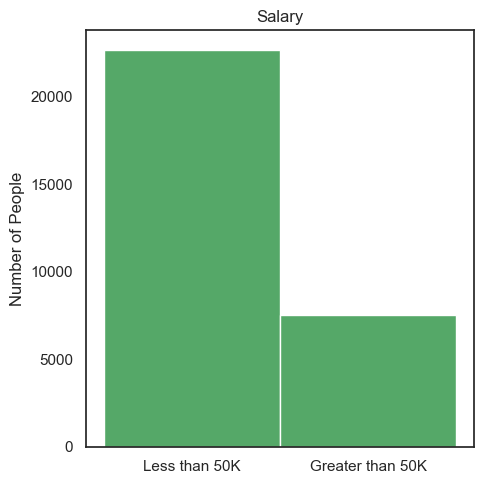
\includegraphics[scale = 0.39]{figs/histograms/ADULT.png}}%
\hspace{8pt}%
\subfigure[b]{%
\label{fig:ex3-b}%
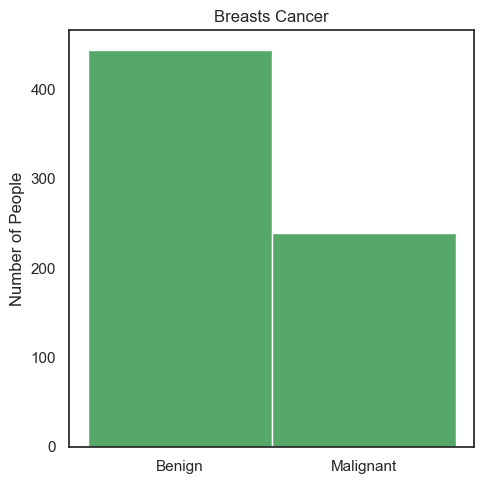
\includegraphics[scale = 0.39]{figs/histograms/BREAST_CANCER_DIAGNOSIS.png}} \\
\subfigure[c]{%
\label{fig:ex3-c}%
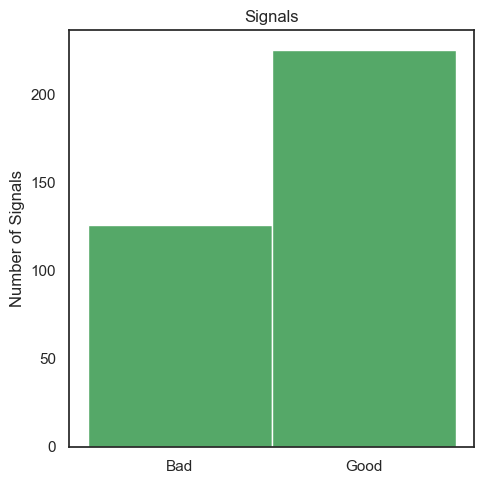
\includegraphics[scale = 0.39]{figs/histograms/IONOSPHERE.png}}%
\hspace{8pt}%
\subfigure[d]{%
\label{fig:ex3-d}%
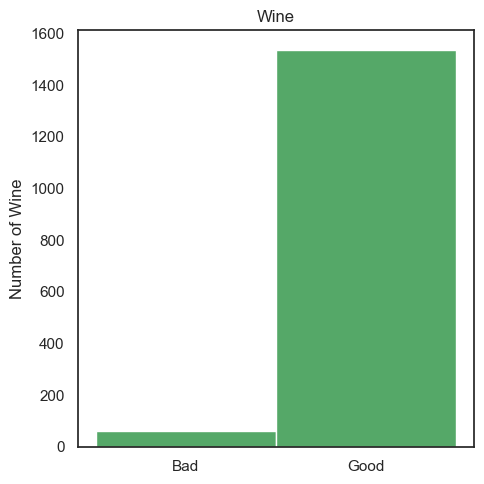
\includegraphics[scale = 0.39]{figs/histograms/WINE_QUALITY.png}}%
\caption[Distributions of the positive vs.
negative classes (histogram).]{Distributions of the positive vs.
negative classes (histogram):
\subref{a} Adult;
\subref{b} Breast Cancer Diagnosis;
\subref{c} Ionosphere; and,
\subref{d} Wine Quality.}%
\label{fig:ex3}%
\end{figure}

\begin{figure}%
\centering
\subfigure[a]{%
\label{fig:ex3-a}%
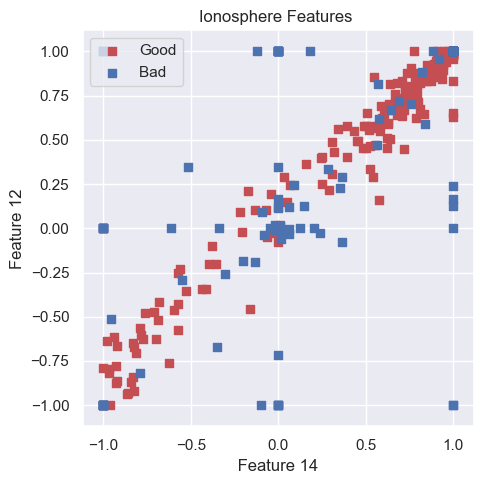
\includegraphics[scale = 0.39]{figs/feature_correlations/IONOSPHERE_high_corr_features_14_12.png}}%
\hspace{8pt}%
\subfigure[b]{%
\label{fig:ex3-b}%
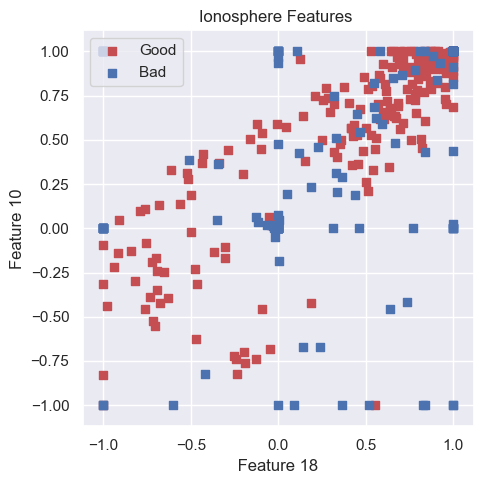
\includegraphics[scale = 0.39]{figs/feature_correlations/IONOSPHERE_low_corr_features_18_10.png}} \\
\subfigure[c]{%
\label{fig:ex3-c}%
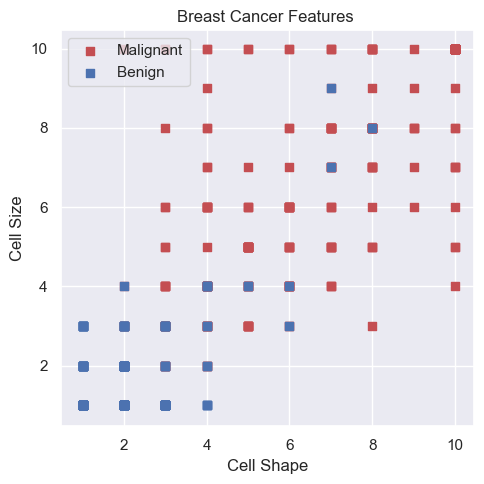
\includegraphics[scale = 0.39]{figs/feature_correlations/BREAST_CANCER_DIAGNOSIS_high_corr_3_2.png}}%
\hspace{8pt}%
\subfigure[d]{%
\label{fig:ex3-d}%
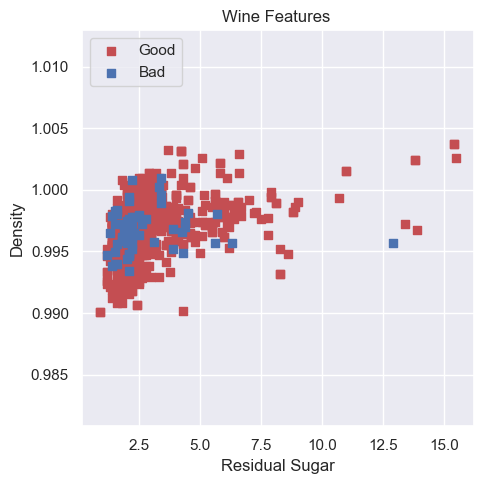
\includegraphics[scale = 0.39]{figs/feature_correlations/WINE_QUALITY_high_corr_features_3_7.png}}%
\caption[Some correlations between
the features.]{Some correlations between
the features.:
\subref{a} Ionosphere (High correlation between features 14 and 12);
\subref{b} Ionosphere (Low correlation between features 18 and 10);
\subref{c} Breast Cancer Diagnosis High correlation between features 3 and 2);
\subref{d} Wine Quality (High correlation between features 2 and 7).}%
\label{fig:ex3}%
\end{figure}

\subsection{Output Labels}

Since we are studying binary classification tasks, we needed to be sure that each dataset only outputs two possible labels. This is true for all datasets, except the Wine Quality one, which outputs a number from 1 to 10. We converted that dataset to a binary task by changing its output to 0 where the original value was less than or equal to 5 and 1 otherwise. We also computed the distributions of the two classes for each dataset and summarize it in Figure \ref{fig:output_ratio}.

\begin{figure}%
\centering
\subfigure[a]{%
\label{fig:ex3-a}%
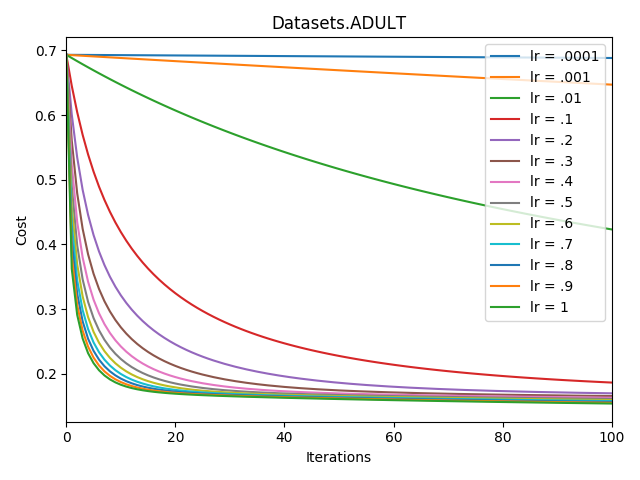
\includegraphics[scale = 0.23]{figs/cost_vs_iterations/ADULT.png}}%
\hspace{8pt}%
\subfigure[b]{%
\label{fig:ex3-b}%
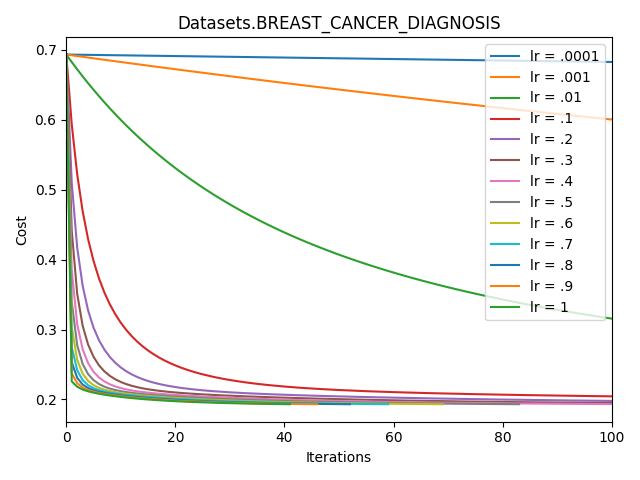
\includegraphics[scale = 0.23]{figs/cost_vs_iterations/BREAST_CANCER_DIAGNOSIS.png}} \\
\subfigure[c]{%
\label{fig:ex3-c}%
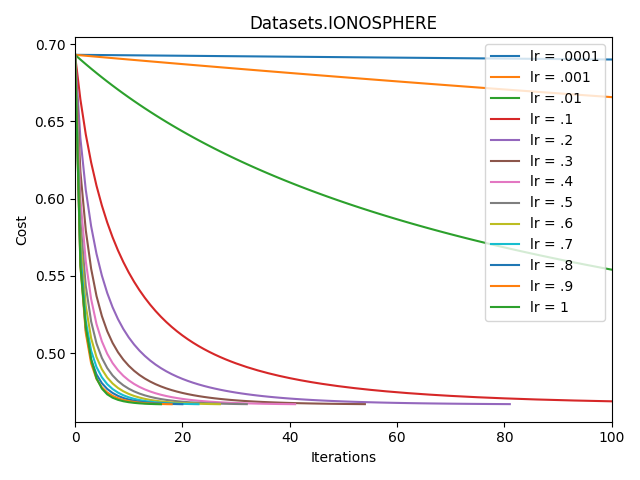
\includegraphics[scale = 0.23]{figs/cost_vs_iterations/IONOSPHERE.png}}%
\hspace{8pt}%
\subfigure[d]{%
\label{fig:ex3-d}%
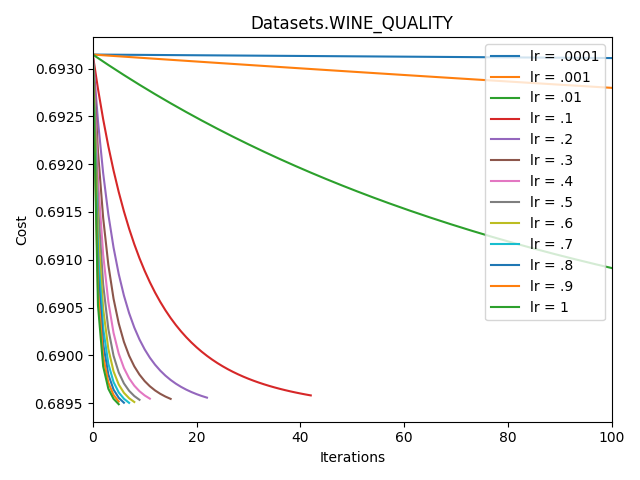
\includegraphics[scale = 0.23]{figs/cost_vs_iterations/WINE_QUALITY.png}}%
\caption[Testing different learning rates for gradient descent applied to logistic regression. Using a threshold for change in the value of the cost function as termination criteria, and plot the accuracy on train/validation set as a function of iterations of gradient descent.]{Testing different learning rates for gradient descent applied to logistic regression. Using a threshold for change in the value of the cost function as termination criteria, and plot the accuracy on train/validation set as a function of iterations of gradient descent.:
\subref{a} Adult;
\subref{b} Breast Cancer Diagnosis;
\subref{c} Ionosphere; and,
\subref{d} Wine Quality.}%
\label{fig:ex3}%
\end{figure}

\subsection{Missing Data and Malformed Features}

The Adult and Breast Cancer Diagnosis datasets have points with missing values for some of the features, represented by the '?' symbol. We decided to remove those points. We also found some malformed features and irrelevant features:

\begin{itemize}
    \item In the Ionosphere dataset 89.2\% of the values of the first feature and all the values of the second feature are zero
    \item In the Adult dataset the columns labeled "capital-gain" and "capital-loss" are also mostly composed of zeros (91.7\% and 95.3\% respectively)
    \item The first feature of the Breast Cancer dataset is the sample code number, which has no influence if the cancer is benign or malignant
\end{itemize}

We decided to remove those features completely.

\subsection{Continuous Fetures}

All features in the Ionosphere, Breast Cancer Diagnosis and Wine Quality datasets and 6 features in the Adult dataset are continuous. We plotted histograms and computed basic statistics for each of them in order to understand their distribution. \textbf{All features in the Wine Quality dataset and many features in the other datasets have a distribution similar to Gaussian. The other features have a multimodal distribution.} Figure \ref{fig:histograms} shows the plots of some of the figures. We also applied stardardization to make the so the data has similar scales.

\subsetion{Categorical Features}

The Adult dataset have 8 categorical features. We applied one-hot encoding to convert those values to numeric.

\subsection{Correlation between features}

\textbf{We draw heatmaps of feature versus feature to understand how they are correlated to each other. We found out that some of the features are highly correlated with other ones. Figure \ref{fig:heatmap} shows the heatmaps for all datasets}

\begin{figure}%
\centering
\subfigure[a]{%
\label{fig:ex3-a}%
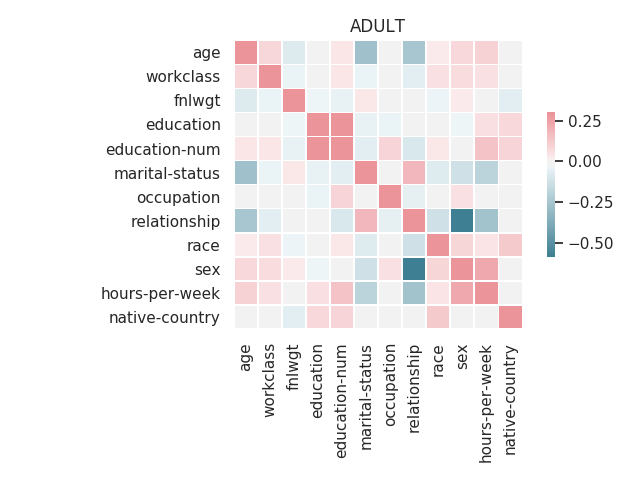
\includegraphics[scale = 0.39]{figs/heatmaps/ADULT.png}}%
\hspace{8pt}%
\subfigure[b]{%
\label{fig:ex3-b}%
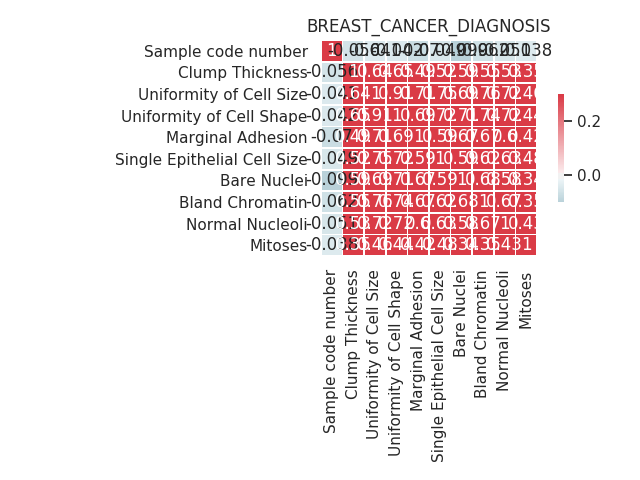
\includegraphics[scale = 0.39]{figs/heatmaps/BREAST_CANCER_DIAGNOSIS.png}} \\
\subfigure[c]{%
\label{fig:ex3-c}%
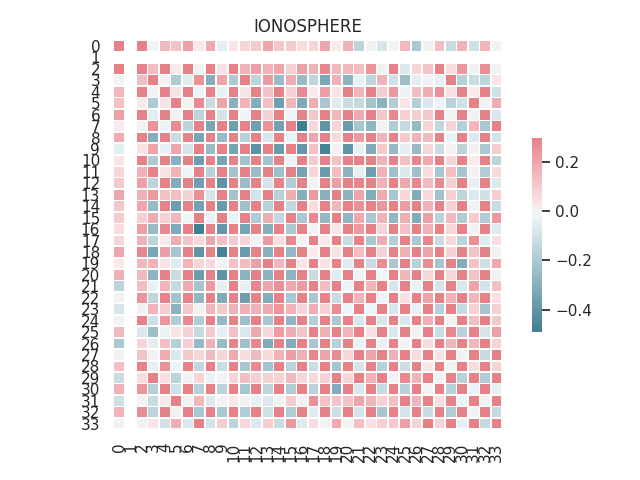
\includegraphics[scale = 0.39]{figs/heatmaps/IONOSPHERE.png}}%
\hspace{8pt}%
\subfigure[d]{%
\label{fig:ex3-d}%
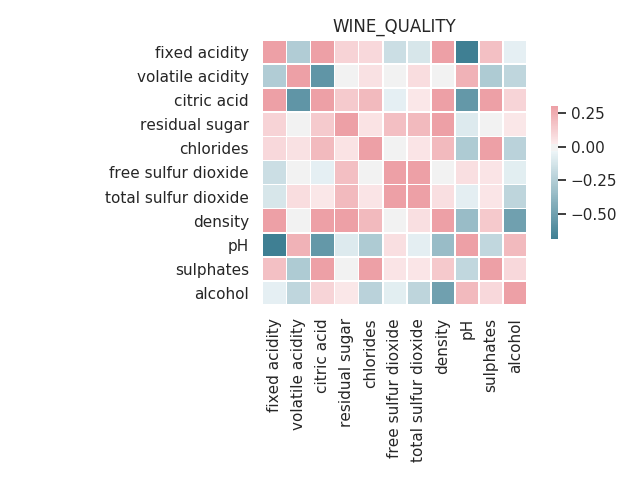
\includegraphics[scale = 0.39]{figs/heatmaps/WINE_QUALITY.png}}%
\caption[Dataset heatmaps (correlation matrix).]{Dataset heatmaps (correlation matrix):
\subref{a} Adult;
\subref{b} Breast Cancer Diagnosis;
\subref{c} Ionosphere; and,
\subref{d} Wine Quality.}%
\label{fig:ex3}%
\end{figure}

\section{Results}
\label{section:results}

\paragraph{assignment} Describe the results of all the experiments mentioned in Task 3 (at a minimum) as well as any other interesting results you find. At a minimum you must report:

\begin{enumerate}
    \item A discussion of how the logistic regression performance (e.g., convergence speed) depends on the learning rate. (Note: a figure would be an ideal way to report these results).
    \item A comparison of the accuracy of naive Bayes and logistic regression on both datasets.
    \item Results demonstrating that the feature subset and/or new features you used improved performance.
\end{enumerate}

\begin{figure}%
\centering
\subfigure[a]{%
\label{fig:ex3-a}%
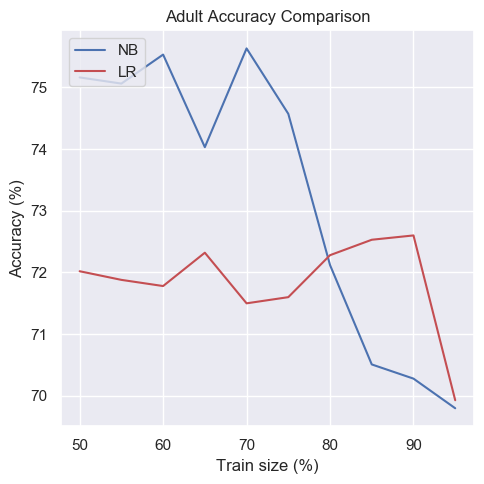
\includegraphics[scale = 0.39]{figs/accuracy_vs_trainingsize/ADULT.png}}%
\hspace{8pt}%
\subfigure[b]{%
\label{fig:ex3-b}%
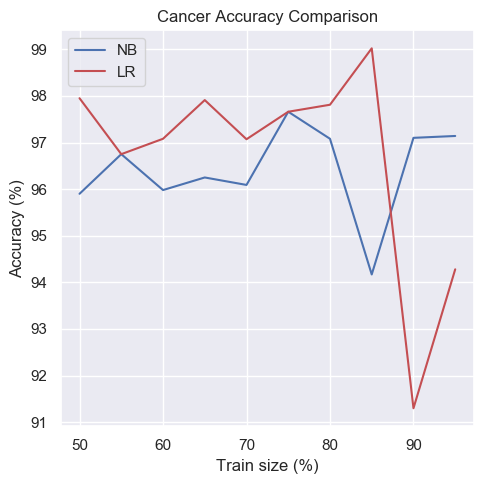
\includegraphics[scale = 0.39]{figs/accuracy_vs_trainingsize/BREAST_CANCER_DIAGNOSIS.png}} \\
\subfigure[c]{%
\label{fig:ex3-c}%
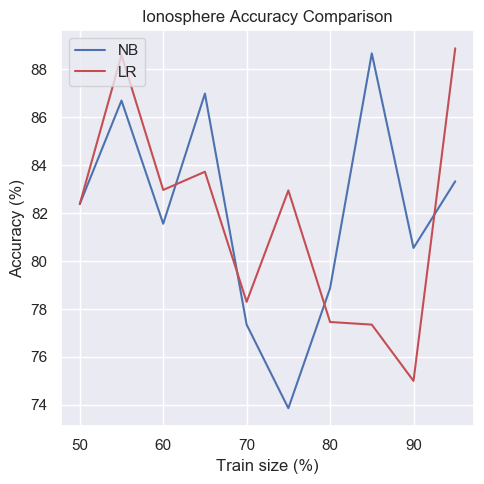
\includegraphics[scale = 0.39]{figs/accuracy_vs_trainingsize/IONOSPHERE.png}}%
\hspace{8pt}%
\subfigure[d]{%
\label{fig:ex3-d}%
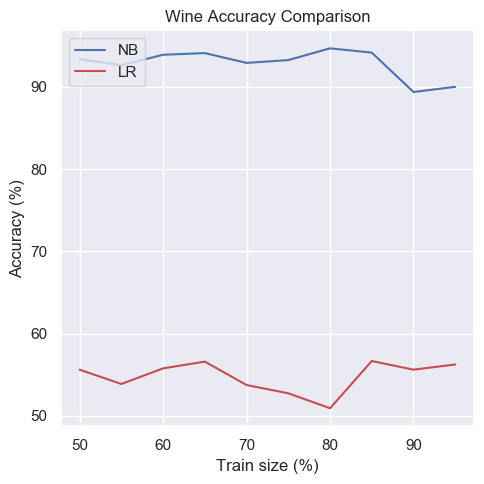
\includegraphics[scale = 0.39]{figs/accuracy_vs_trainingsize/WINE_QUALITY.png}}%
\caption[Comparing the accuracy of the two models (LR and NB as a function of the size of dataset (by controlling the training size).]{Compare the accuracy of the two models as a function of the size of dataset (by controlling the training size):
\subref{a} Adult;
\subref{b} Breast Cancer Diagnosis;
\subref{c} Ionosphere; and,
\subref{d} Wine Quality.}%
\label{fig:ex3}%
\end{figure}

\begin{table}
  \caption{Testing accuracy of Linear Regression (LR) and Naive Bayes (NB) versus the corresponding scikit-learn implementations (SK-LR and SK-NB) for each of the four datasets}
  \label{table:accuracy}
  \centering
  \begin{tabular}{lllll}
    \toprule
    Dataset       & LR   & NB   & SK-LR & SK-NB \\
    \midrule
    Ionosphere    & 10\% & 10\% & 10\% & 10\%  \\
    Adult         & 10\% & 10\% & 10\% & 10\%  \\
    Wine Quality  & 10\% & 10\% & 10\% & 10\%  \\
    Breast Cancer & 10\% & 10\% & 10\% & 10\%  \\
    \bottomrule
  \end{tabular}
\end{table}

\section{Discussion and Conclusion}
\label{section:discussion}

\paragraph{assignment} Summarize the key takeaways from the project and possibly directions for future investigation.

\section{Statement of Contributions}
\label{section:contributions}

\paragraph{assignment} State the breakdown of the workload across the team members.

Ege worked on the visualization and analysis of the datasets, and implemented the \textit{evaluate\_acc} function. Rafael implemented the machine learning models. Ramon worked on the preprocessing of data, provided the \textit{sklearn} implementation that we used as benchmark and developed the k-fold cross validation script.

\subsection{Sample Figure and Table}

Use this code as an example to include figures and tables.

\begin{table}
  \caption{Sample table title}
  \label{sample-table}
  \centering
  \begin{tabular}{lll}
    \toprule
    \multicolumn{2}{c}{Part}                   \\
    \cmidrule(r){1-2}
    Name     & Description     & Size ($\mu$m) \\
    \midrule
    Dendrite & Input terminal  & $\sim$100     \\
    Axon     & Output terminal & $\sim$10      \\
    Soma     & Cell body       & up to $10^6$  \\
    \bottomrule
  \end{tabular}
\end{table}

\section*{References}

References follow the acknowledgments. Use unnumbered first-level heading for
the references. Any choice of citation style is acceptable as long as you are
consistent. It is permissible to reduce the font size to \verb+small+ (9 point)
when listing the references. {\bf Remember that you can use more than eight
  pages as long as the additional pages contain \emph{only} cited references.}
\medskip

\small

\begin{thebibliography}{9}
\bibitem{ionosphere} 
V. G. Sigillito, S. P. Wing, L. V. Hutton, and K. B.
Baker 
\textit{ “Classification of radar returns from the
ionosphere using neural networks,”} 
 Johns Hopkins APL Tech. Dig. Applied Phys. Lab., 1989. 
 
 \bibitem{adult} 
Ron Kohavi
\textit{ “Scaling Up the Accuracy of Naive Bayes Classifier: a Decision Tree Hybrid”} 
 Johns Hopkins APL Tech. Dig. Applied Phys. Lab., 1996. 

 \bibitem{wine} 
 P. Cortez, A. Cerdeira, F. Almeida, T. Matos and J. Reis. 
\textit{ “Modeling wine preferences by data mining from physicochemical properties.”} 
In Decision Support Systems, Elsevier, 47(4):547-553. ISSN: 0167-9236.

\end{thebibliography}

% @article{Cortez2009ModelingWP,
%   title={Modeling wine preferences by data mining from physicochemical properties},
%   author={Paulo Cortez and Ant{\'o}nio Cerdeira and Fernando Almeida and Telmo Matos and Jos{\'e} Reis},
%   journal={Decision Support Systems},
%   year={2009},
%   volume={47},
%   pages={547-553}
% }

% @inproceedings{Sigillito1989ClassificationOR,
%   title={Classification of radar returns from the ionosphere using neural networks},
%   author={Vincent G. Sigillito and Simon Wing and Larrie V. Hutton and Kevin Baker},
%   year={1989}
% }

% @INPROCEEDINGS{Kohavi96scalingup,
%     author = {Ron Kohavi},
%     title = {Scaling Up the Accuracy of Naive-Bayes Classifiers: a Decision-Tree Hybrid},
%     booktitle = {PROCEEDINGS OF THE SECOND INTERNATIONAL CONFERENCE ON KNOWLEDGE DISCOVERY AND DATA MINING},
%     year = {1996},
%     pages = {202--207},
%     publisher = {AAAI Press}
% }
\end{thebibliography}

\end{document}